\section{Motivation}
\begin{figure*}[t]
	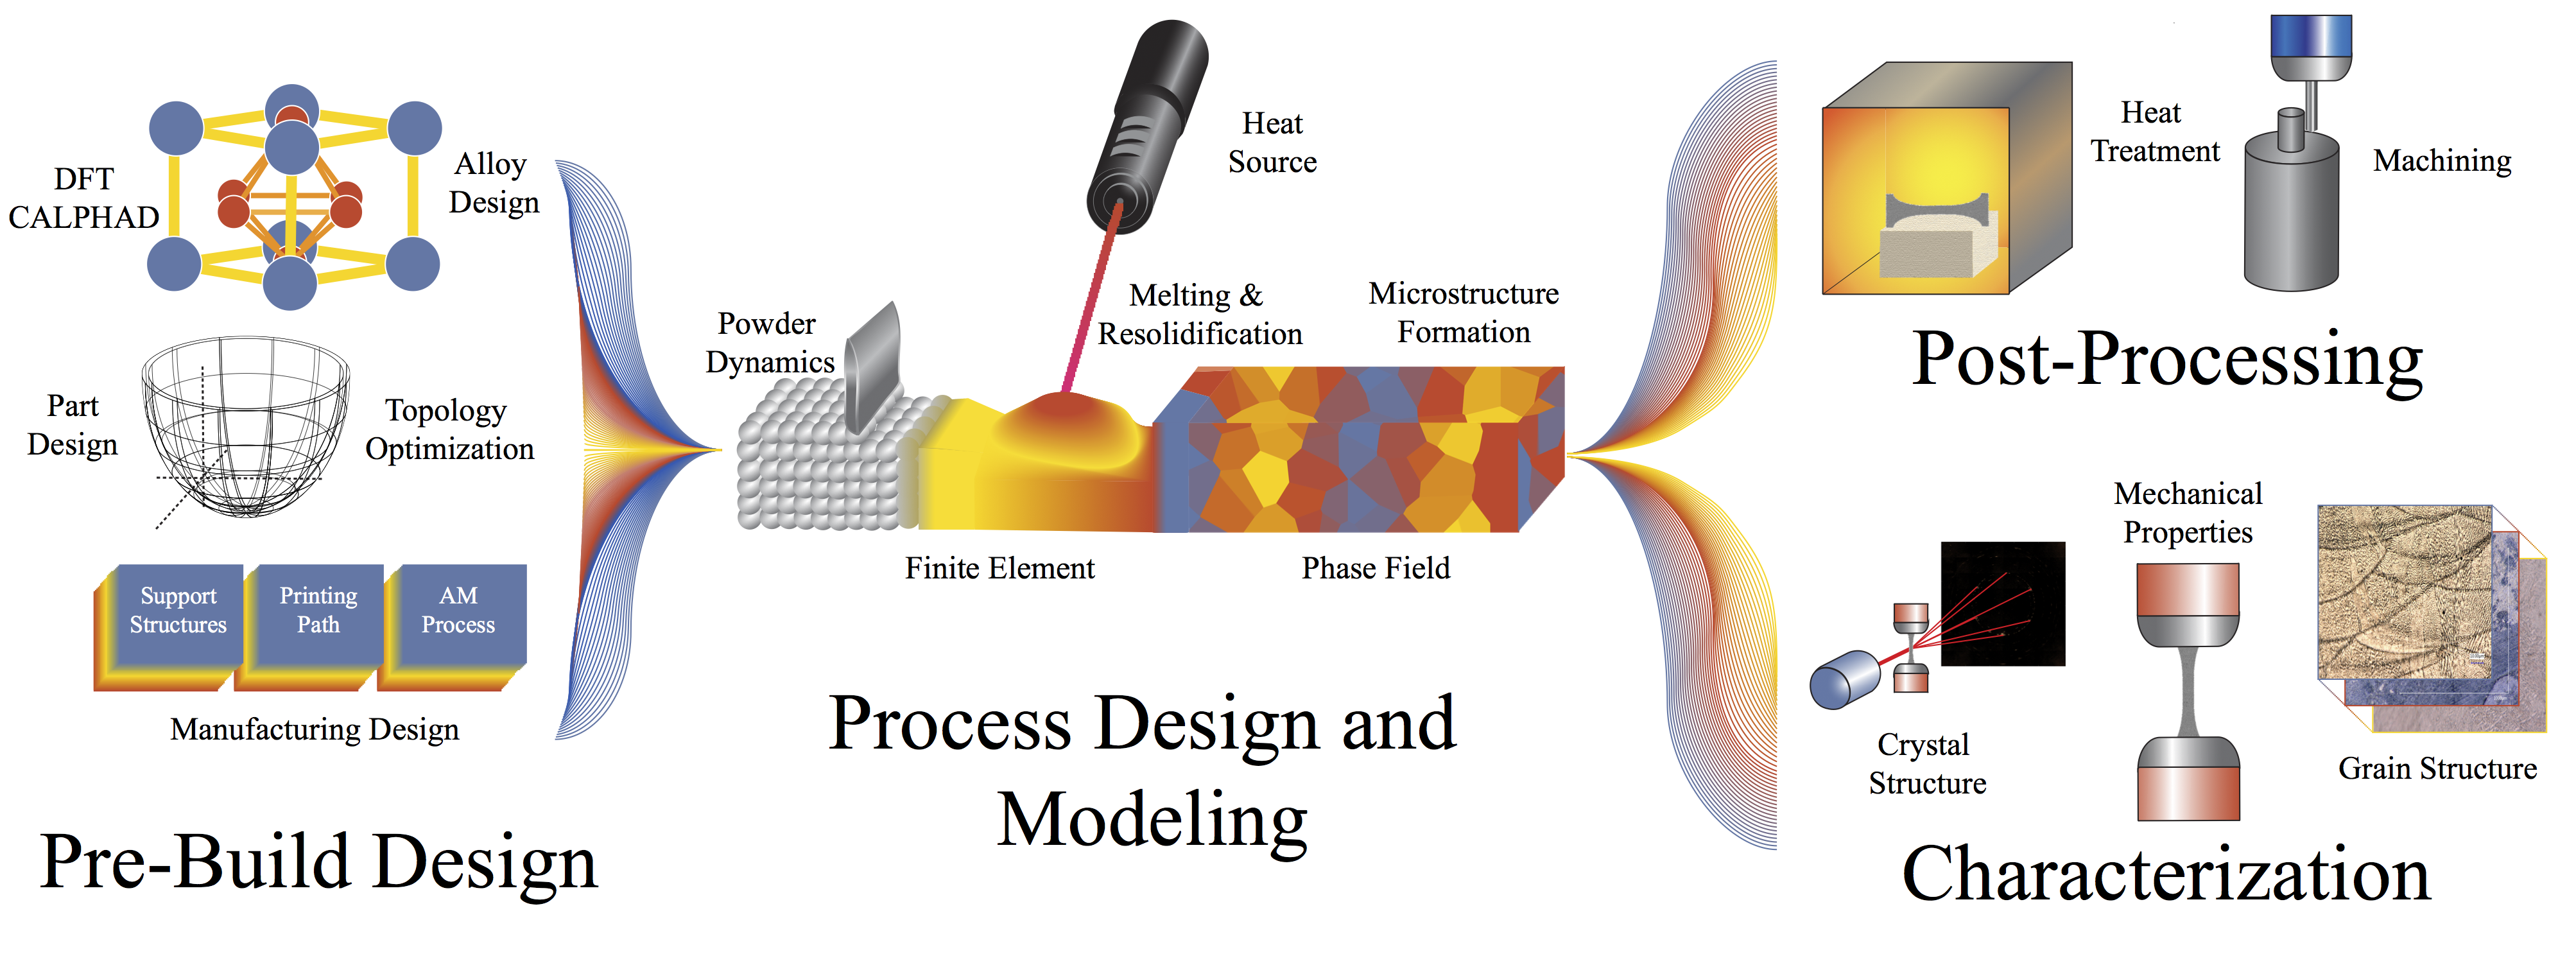
\includegraphics[width=1\linewidth]{Images/AMgene.png}
	\caption{The design space of additive manufacturing. The study and use of AM generates data at all length and time scales throughout the manufacturing pipeline, from pre-process engineering, to process monitoring, to post-manufacture characterization and implementation. This data can be implemented in a larger integrated computational materials engineering ecosystem that optimizes process design at a single step within the manufacturing pipeline and links materials properties across different steps in the pipeline.}
	\label{AMgene}
\end{figure*}

Metals additive manufacturing (AM) enables paradigm shifts in how metallic products are manufactured, provides versatility in the type and design of parts, it enables materials and parts to be produced by a single machine and enables novelty in the microstructure design of the parts resulting in new and enhanced properties. Although decades of scientific and engineering work in industry, academia, and government have resulted in the commercialization of AM, there have been significant roadblocks to fully realize AM's potential, particularly in the control of consistency and quality in part production and in the development of materials amenable to the AM process. Integrated Computational Materials Engineering (ICME) approaches have proven to accelerate development and adoption of materials technologies. Traditionally ICME approaches incorporate physics-based experiments and simulations across many fields and scientific methods. However, for metals AM, much of the physics are still being discovered, hence physics-first approaches to ICME are still immature. The diverse array of promises and problems in AM has resulted in a field of study which is rich with data -- so much so that our ability to store and analyze the data is challenged. At the same time, this wealth of data is motivating a paradigm shift in ICME toward data-driven, statistics based machine learning ICME approaches. 

\subsection{Background}
The 20th century saw the maturation of materials science and engineering as a field of study, enabling targeted materials discoveries and innovations for specific applications. Over the past decades, materials development has greatly accelerated by formulating materials problems through the process-structure-property-performance paradigm \cite{Olson2000, Panchal2013}. 

The process-structure-property-performance (PSPP) paradigm is a core philosophy in materials science that governs how the manufacturing of a material determines its ability to be used in different engineering applications. First introduced by Olson in 2000 \cite{Olson2000}, the PSPP relationships break down materials development into four key areas of scientific and engineering interest. Various phenomenon and measurements of interest for an AM-specific PSPP paradigm can be seen in Figure \ref{PSPP}.

The \textbf{processing} of a material is the thermal, mechanical, and chemical behaviors experienced by an AM part throughout the duration of its manufacture. The design parameters chosen, and subsequent thermal history experienced by the part, are most often thought of as an AM part's processing history. Controllable machine parameters like energy density, the order in which part layers are manufactured, or the location of parts on the build plate are determining factors in the part's processing. The actual processing history, however, is better described by the thermal history of the build volume, both during manufacture and post-processing, the mechanical forces it experiences, and any chemical reactions that occur in or on the part. Processing \textit{routes} are often discussed in AM and typically refer to beneficial or detrimental processing histories that impact the part's structure.

The \textbf{structure} of a material is a wide-ranging concept that spans all length scales of materials science. Structure can refer to the crystallographic structure of a metal, at the atomic scale, to the morphology and orientation of metal grains, at the mesoscale, to the geometry of the part being manufactured, at the macroscale. \textit{Micro}structure is a term often used in materials science referring to a specific subset of the material structure. Microstructure for metals most commonly refers to grain and sub-grain level information like material phases, grain morphologies, texture, and any defects like pores or cracks that might be present. The structures encompassing microstructure are so often referred to because they are a primary determinant of a material's properties. 

The \textbf{properties} of a material are characteristics which determine its quality or qualification of use in an engineering application. Properties for AM parts are also wide-ranging and the `properties of interest' vary depending on the desired engineering application of the part. Mechanical properties are some of the most studied material properties in AM because AM has a lot to offer for improving mechanical performance of parts. However, AM currently has equally as many drawbacks for mechanical properties which is why it has requires so much scientific and engineering attention. Other properties of interest include thermal properties, such as the heat transfer through an AM part, chemical properties, like corrosion resistance, and optical properties, like reflectance. Measuring material properties are the first step in evaluating an engineering part's performance.

The \textbf{performance} of a part is its ability to be successfully implemented in an engineering application. Performance can be viewed through the lifetime of an AM part in deployment. While an AM part may have improved static properties over traditionally manufactured metals, it is not necessarily guaranteed to be more useful in an application. A common performance metric for materials is fatigue life, or the ability of a part to consistently perform over many application cycles. Other performance characteristics include thermal and chemical stability in dynamic environments. Performance can also be thought of as the environment in which an AM part will be employed, including the mechanical, thermal, chemical, etc. forces it will experience during use.

The process-structure-property-performance paradigm has been presented (and is often though of) as a cause-and-effect relationship between the different levels. In reality, it is a complex relationship with many materials models/theories that interconnect and bridge each level. Different processing routes will result in different properties, the performance of a part can change its structure, the structure of a material can determine its performance, and so on. The ICME approach to materials science is focused on modeling, bridging, and predicting relationships throughout the PSPP paradigm.

Computational materials science has enabled the prediction of microstructure from processing and of properties from microstructure, reducing the need for costly and time consuming experimentation. Today ICME approaches tightly integrate physics-based computational models into the industrial design process, allowing the desired performance requirements of a part to guide the design of a novel material. Examples specific to alloys include low-RE Ni superalloys for better turbine performance \cite{Pollock2016} and lower cost and radioactive element free Ferrium S53 alloy designed for corrosion-resistant landing gears \cite{Olson2014}. Both cases took materials innovation timelines from decades to years, demonstrating the practical capability of designing new materials within an industrial product timeframe. Generalizing this capability to more industries and further accelerating the process is the primary goal of the Materials Genome Initiative (MGI) \cite{MGI}.

Many of the current limitations of AM are difficult to solve with existing physics-based ICME approaches. The physics of AM processes are more complex than traditional casting methods as they involve rapid solidification, vaporization and ingestion of volatile elements, and complex thermal history that consists of dozens of heating and cooling cycles, each one different. Furthermore, all of these additional complexities vary from one location to another within a part and from part to part within a build volume. For AM, physics-based ICME tools have been mostly developed through attempts to bootstrap legacy models formulated for traditional manufacturing of alloys to AM data, with some success. However, the lower cost and time barrier to entry for performing AM has enabled the rapid accumulation of experimental data, enabling a high-throughput approach for finding optimized AM processing methods and parameters of existing alloys. As such, current AM materials development is largely combinatorial and consists of adopting AM processing of legacy alloys that were developed for other types of manufacturing using extensive design of experiments.

It is with awareness of the grand amounts of data being generated in AM that machine learning (ML) can accelerate AM innovations and their commercialization. ML as a method for model development has shown wide application in recent years, including finance \cite{Bose2001}, molecule design for genomics, chemistry and pharmacology \cite{Gomez-Bombarelli2018}, social networking \cite{Brusilovsky2007} and, most importantly to this review, materials science. Still, the use of ML in materials science has been relatively limited for a variety of reasons, especially the lack of large curated datasets amenable to existing ML methodologies. Through the work done under the MGI, this data limitation was identified as a primary impediment to future materials innovations \cite{MGI}. In response, there has been significant recent investment in infrastructure development for materials databases suitable for data informatics innovations. It is now recognized and accepted that ML frameworks can couple legacy physics-based ICME tools with experimental data to produce more accurate process-structure-property models and to automate the iteration of designed experiments for model improvement and optimized materials \cite{Rajan2005, Agrawal2016, Butler2018, Ball2019}

We proceed to review how the paradigm shift from physics-based to data-driven ICME approaches can be made through solving metals AM challenges. We begin by phrasing terms and ideas from additive manufacturing in ways that are compatible with machine learning. We provide basics of machine learning algorithms and how they can be interpreted in an additive manufacturing study. Following this introduction to using ML for AM problems, we review other uses of machine learning in materials science and state the uses of such approaches for solving AM challenges. We conclude with an outlook for how database-driven design of materials for AM can accelerate material creation and part qualification.
